\chapter{The FNAL Recycler Ring}

The Fermilab Recycler Ring (RR) is one of the circular accelerators located in the Fermilab Accelerator Complex. It was originally designed to store and accumulate antiprotons that remained from a Tevatron event \cite{rr0}. The recycling of antiprotons was deemed ineffective and was never operationally implemented \cite{rrnagaitsev}. Since 2011, the RR has been repurposed to act as a pre-injector to the Main Injector (MI) by storing and accumulating protons \cite{rr1}. It is worth pointing out, that the MI and the RR share the same tunnel, which has a circumference of 3.319 km (2.062 mi).

The MI/RR complex is fed protons by the Proton Source, which by itself consists of the Pre-Accelerator, the Linear Accelerator (Linac), and the Booster. The Pre-Accelerator systems provide $H^-$ ions to the Linac, where they are accelerated to an energy of 400 MeV. After this, the beam is injected into the Booster, which is a rapid-cycling synchrotron operating at a 15 Hz repetition rate. During this injection process, the $H^-$ beam passes through a carbon stripping foil, and it incorporates to the circulating proton beam. The Booster ramps the energy up from 400 MeV to 8 GeV. This 8 GeV proton beam can either go to the Booster Neutrino Experiments or get injected into the Recycler Ring. Once in RR the beam has two possible destinations: 1) high energy neutrino experiments through MI or 2) Muon Campus. For the latter, proton beam gets rebunched from 53 MHz to 2.5 MHz and transported to Muon Campus. For high energy neutrino experiments, the proton beam gets slip-stacked, hence doubling the intensity that gets injected into Main Injector. Once in MI, the beam is accelerated to 120 GeV and sent to the NuMI (Neutrinos at the Main Injector) beam facility \cite{rr1, rrnagaitsev, numi1}. A description of the accelerator complex is shown in figure \ref{fig:fnal}, including the experimental beamlines which feed neutrino, muon and fixed target experiments.

The work done for this thesis focuses on the Recycler Ring. The following chapter starts by giving a general description for the operation and physics of the Recycler Ring. The next sections introduce and motivate the compensation of third order resonances for high intensity operation.\\     

\begin{figure}[]
   \centering
   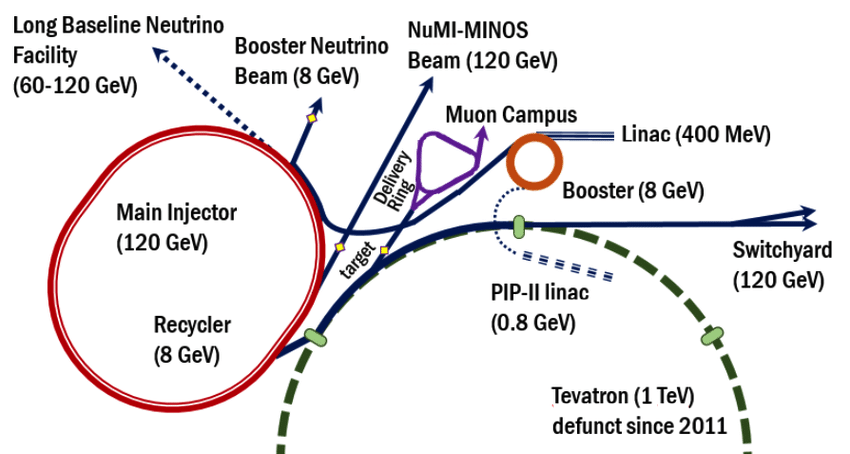
\includegraphics[width=\columnwidth]{chapter1/FNAL.png}
   \caption{The past (Tevatron), present and future (PIP-II and LBNF) of the FNAL Accelerator Complex, taken from [3].}
   \label{fig:fnal}
\end{figure}

\section{General Specifications}

The RR is a permanent magnet storage ring operating at a fixed momentum of 8.835 Gev/c.
\cite{pipII1}

\begin{table}[]
\centering
\caption{Typical Recycler Ring properties for beam sent to NuMI}
\label{tab:rrparams}
\begin{tabular}{@{}ccc@{}}
\toprule
\textbf{Parameter}          & \textbf{Value}                             & \textbf{Unit} \\ \midrule
Circumference               & 3319                                       & m             \\
Momentum                    & 8.835                                      & GeV/c         \\
RF Frequency                & 52.8                                       & MHz           \\
RF Voltage                  & 80                                         & kV            \\
Harmonic Number             & 588                                        &               \\
Synchrotron Tune            & 0.0028                                     &               \\
Slip Factor                 & -8.6 $\times$ 10$^{-3}$                    &               \\
Superperiodicity            & 2                                          &               \\
Horizontal Tune             & 25.43                                      &               \\
Vertical Tune               & 24.445                                     &               \\
Horizontal Chromaticity     & -6                                         &               \\
Vertical Chromaticity       & -7                                         &               \\
95\% Normalized Emittance   & 15                                         & $\pi$ mm mrad \\
95\% Longitudinal Emittance & 0.08                                       & eV s          \\
Intensity                   & $5\times10^{10}$, $8\times10^{10}$ (PIP-II) & ppb           \\
MI Ramp Time                & 1.333, 1.133, 1.067                        & s             \\
Booster Frequency           & 15, 20 (PIP-II)                            & Hz            \\ \bottomrule
\end{tabular}
\end{table}

\section{Tune Diagram and Resonances}

\section{High Intensity and Tune Footprint}

